\index{Event generators|see{Monte Carlo}}
\index{Monte Carlo!Event generators}
\section{Monte Carlo Event Generators \label{sec:MC}}

In this section, we discuss the physics of Monte Carlo event generators and
their mathematical foundations, at an introductory level. We shall attempt
to convey the main ideas as clearly as possible without burying them
in an avalanche of technical details. References to
more detailed discussions are included where applicable.
We assume the reader is already familiar with the contents of the
preceding section on hard processes. 

The task of a Monte Carlo event generator is to calculate
everything that happens in a high-energy collision, from the hard
short-distance physics to the long wavelengths of hadronisation and
hadron decays. Obviously, this requires some compromises to be
made. General-purpose generators like \Hw~\cite{Corcella:2000bw,Bahr:2008pv,Bellm:2015jjp},
\Py~\cite{Sjostrand:2006za,Sjostrand:2014zea}, and \Sh~\cite{Gleisberg:2008ta}, 
start from low-order (LO or NLO) descriptions of the perturbative hard physics
and then attempt to include the ``most significant'' corrections, such
as higher-order matrix-element corrections and parton showers,
resonance decays and finite-width effects, 
underlying event, beam remnants, hadronisation, and hadron
decays. Each of them had slightly different origins, which carries
through to the emphasis placed on various physics aspects today:
\begin{itemize}
\item \Py. \index{PYTHIA} 
Successor to \textsc{Jetset} (begun in 1978). Originated in
hadronisation studies. Main feature: the Lund string fragmentation model. 
\item \Hw. \index{HERWIG}
\index{Angular ordering}
Successor to \textsc{Earwig} (begun in 1984). Originated in
perturbative coherence studies. Main feature:
angular-ordered parton showers.
\item \Sh. \index{SHERPA}
Begun in 2000. Originated in studies of the matching of 
hard-emission matrix elements with parton showers. Main feature: 
CKKW matching. 
\end{itemize}
There is also a large number of more specialised generators, mainly
for hard processes within and beyond the SM, 
a few that offer alternative shower
models, and ones specializing in soft-inclusive and/or heavy-ion
physics.

An important aspect of contemporary generators is the
ability to combine specialised ones with general-purpose ones, via interfaces. 
The most common interface
between partonic hard-process and parton-shower generators is  the
\index{Les Houches Event Files|see{LHEF}}%
\index{LHEF}%
Les Houches Event File (LHEF) standard, defined
in~\cite{Boos:2001cv,Alwall:2006yp} and ``spoken'' by most modern
generator tools. For interfaces to experimental analysis
packages (like \textsc{Rivet}~\cite{Buckley:2010ar}) 
and detector simulations
(like \textsc{Geant}~\cite{Agostinelli:2002hh}), 
typically the HepMC standard is used~\cite{Dobbs:2001ck}. 

Hard processes were the topic
of \secRef{sec:pQCD}. In this section, we shall focus
mainly on parton showers, with some brief comments on resonance
decays at the end. 
\SecRef{sec:matching} then concerns the matching of matrix elements 
and parton showers. Finally, models of hadronisation and the
underlying event  are the topic of \secRef{sec:soft}.

Several of the discussions below rely on material from the section on Monte
Carlo Event Generators in the PDG Review of Particle Physics~\cite{pdg2012} and
on the more comprehensive  
\index{MCnet review}%
review by the {\sl MCnet} collaboration 
in \cite{Buckley:2011ms}. The latter also contains brief
descriptions of the  
physics implementations of each of the main general-purpose event
generators on the 
market, together with a guide on how to use (and not use) them 
in various connections, and a collection of comparisons to important
experimental 
distributions. We highly recommend readers to obtain a copy of that
review, as it is the most comprehensive and up-to-date review of event
generators currently available. Another useful and pedagogical review
on event generators is contained in the 2006 ESHEP lectures
by Torbj\"orn Sj\"ostrand \cite{Sjostrand:2006su}, with a more recent update in
\cite{Sjostrand:2009ad}. 

\index{Monte Carlo!Integration}
\subsection{The Monte Carlo Method}
A ubiquitous problem in fundamental physics is the following:
given a source located some distance from a detector, predict the
number of counts that should be observed within the solid angle spanned
by the detector (or within a bin of its phase-space acceptance), as a
function of the properties of the source, the intervening medium,
and the efficiency of the detector. Essentially, the task is to
compute integrals of the form
\begin{equation}
N_\mrm{Count}(\Delta\Omega) \ = \ \int_{\Delta \Omega} \dd{\Omega} \frac{\dd{\sigma}}{\dd{\Omega}}~,
\end{equation}
with $\dd{\sigma}$ a differential cross section for the process of
interest. 

In particle physics, phase space has three dimensions per final-state 
particle (minus four for overall
four-momentum-conservation). 
Thus, for problems with more than a few outgoing particles, the
dimensionality of phase space increases rapidly. 
At LEP, for instance, the total multiplicity of neutral +
charged hadrons (before weak decays) was typically $\sim$ 30 particles, 
for about 86 dimensions. 

\index{Convergence}%
\index{Numerical integration}%
\index{Monte Carlo!Integration}%
The standard 1D numerical-integration methods 
give very slow convergence rates for
higher-dimensional problems. For illustration, a table of convergence
rates in 1 and $d$ dimensions is given in \tabRef{tab:convergence},
comparing the Trapezoidal (2-point) rule and Simpson's (3-point) rule
to random-number-based Monte Carlo. 
\begin{table}[t]
\centering
\index{Uncertainties!Monte Carlo statistics}%
\index{Monte Carlo!Statistics}%
\index{Monte Carlo!Uncertainties}%
\begin{tabular}{c|cc|c}
\toprule
\mbox{Relative uncertainty with $n$ points} &
1-Dim & $d$-Dim & $n_{\mrm{eval}}$/point \\
\midrule
\mbox{Trapezoidal Rule}  & $1/n^2$ & $1/n^{2/d}$ & $2^d$\\
\mbox{Simpson's Rule}  & $1/n^4$ & $1/n^{4/d}$ & $3^d$\\
\midrule
\mbox{Monte Carlo} & $1/\sqrt{n}$ & $1/\sqrt{n}$& $1$ \\
\bottomrule
\end{tabular}
\caption{Relative uncertainty after $n$ evaluations, in $1$ and $d$
dimensions, for two traditional
numerical integration methods and stochastic Monte Carlo. The 
last column shows the number of function evaluations that are
required per point, in $d$ dimensions. 
\label{tab:convergence}}
\end{table}
In 1D, the $1/n^2$ convergence rate of the 
Trapezoidal rule is much faster than the stochastic $1/\sqrt{n}$ of
random-number Monte Carlo, and
Simpson's rule converges even faster. However, as we go to 
$d$ dimensions, 
the convergence rate of the 
$n$-point rules all degrade with $d$ (while the number of function
evaluations required for each ``point'' simultaneously increases). The
MC convergence rate, on the other hand, remains the simple stochastic 
$1/\sqrt{n}$, independent of $d$, and each point still only requires
one function evaluation. 
\index{Monte Carlo!Integration}%
These are some of
the main reasons that MC is the preferred numerical integration
technique for high-dimensional problems. In addition, the random
phase-space vectors it generates can be re-used in many ways, for
instance as input to iterative solutions, to compute many different
observables simultaneously, and/or to hand ``events'' to propagation
and detector-simulation codes. 

Therefore, virtually
all numerical cross section calculations are based on Monte Carlo
techniques in one form or another, the simplest being the 
\index{Monte Carlo!RAMBO}%
\index{RAMBO}%
\textsc{Rambo} algorithm \cite{Kleiss:1985gy} which can be expressed
in about half a page of code and generates a flat scan over $n$-body
phase space\footnote{Strictly speaking, \textsc{Rambo} is only truly
  uniform for massless particles. Its massive variant makes up for
  phase-space biases by returning weighted momentum configurations.}. 

\index{Infrared divergences}%
However, due to 
the infrared singularities in perturbative QCD, and due to the
presence of short-lived resonances, the functions to be
integrated, $|{\cal{M}}_{F+k}|^2$, can be highly non-uniform,
especially for large $k$.
This implies that we will have to be clever in the way
we sample phase space if we want the integration to converge in any
\index{RAMBO}%
reasonable amount of time --- simple algorithms like \textsc{Rambo} 
quickly become inefficient for $k$ greater than a few. 
To address this bottleneck, 
the simplest step up
from \textsc{Rambo} is to introduce generic (i.e., automated) 
importance-sampling methods, such as offered by the  
\index{Monte Carlo!VEGAS}%
\index{VEGAS|see{Monte Carlo}}%
\textsc{Vegas} algorithm \cite{Lepage:1977sw,Lepage:1980dq}. This is still the
dominant basic technique, although most modern codes do employ several 
additional refinements, such as several different copies of \textsc{Vegas}
running in parallel (multi-channel integration), to further optimise
the sampling.  
Alternatively, a few algorithms incorporate the singularity structure of QCD
explicitly in their phase-space sampling, either by directly generating momenta
distributed according to the leading-order QCD singularities, in a
sort of ``QCD-preweighted'' analog of \textsc{Rambo}, called
\index{SARGE}%
\index{Markov chains}%
\textsc{Sarge} \cite{Draggiotis:2000gm}, or by using all-orders
Markovian parton showers to generate them 
\index{VINCIA}
(\textsc{Vincia} \cite{Giele:2011cb,LopezVillarejo:2011ap,Fischer:2016vfv}).  


\begin{figure}[t]
\centering
\begin{minipage}{0.45\textwidth}
\includegraphics*[scale=0.5]{montecarlo.png}
\end{minipage}
 \hfill  
\index{Convergence}%
\index{Monte Carlo!Convergence}%
\begin{minipage}[c]{0.46\textwidth}\it
``This risk, that convergence is only given with a certain probability,
is inherent in Monte Carlo calculations and is the reason why this
technique was named after the world's most famous gambling
casino. Indeed, the name is doubly appropriate because the style of
gambling in the Monte Carlo casino, not to be confused with the noisy
and tasteless gambling houses of Las Vegas and Reno, is serious and
sophisticated.''
\flushright \color{gray}
F. James, ``Monte Carlo theory and practice'',\\ 
Rept.~Prog.~Phys.~43~(1980)~1145 
\end{minipage}
\caption{{\sl Left:} The casino in Monaco. {\sl Right:} 
\index{Monte Carlo!Monaco}%
extract from \cite{James:1980yn} 
concerning the nature of Monte Carlo techniques.
\label{fig:montecarlo}}
\end{figure}

%%% Insert from slides on basic MC
\index{Convergence}
\index{Monte Carlo!Convergence}
\index{Monte Carlo!Integration}
The price of using random numbers is that we must generalise our
notion of convergence. 
In calculus, we say that a sequence $\{A\}$ \emph{converges} to $B$ if
an $n$ exists for which the difference $|A_{i>n} -B|<\epsilon$ for any
$\epsilon > 0$. In random-number-based techniques, we cannot
completely rule out the possibility of very pathological sequences of
``dice rolls'' leading to large deviations from the true goal, 
hence we are restricted to
say that $\{A\}$ converges to $B$ if an $n$ exists for which \emph{the
probability} for $|A_{i>n} - B| < \epsilon$, for any $\epsilon > 0$,
is greater than $P$, for any $P\in[0,1]$~\cite{James:1980yn}. 
This risk, that convergence
is only given with a certain probability, is the reason why Monte
Carlo techniques were named after the famous casino in Monaco, 
illustrated in \figRef{fig:montecarlo}. 

\index{Parton showers}
\subsection{Theoretical Basis of Parton Showers\label{sec:parton-showers}}

\index{pQCD}
In \secRef{sec:pQCD}, we noted two 
conditions that had to be valid for fixed-order truncations of the
perturbative series to be valid: firstly, the strong coupling
$\alpha_s$ must be small for perturbation theory to be valid at
all. This restricts us to the region in which all scales $Q_i\gg
\Lambda_\mrm{QCD}$. We shall maintain this restriction in this
section, i.e., we are still considering \emph{perturbative QCD}. 
Secondly, however, in order to be allowed to \emph{truncate} the
perturbative 
series, we had to require  $\sigma_{k+1} \ll \sigma_k$, i.e., the
corrections at successive orders must become successively smaller, which --- due
to the enhancements from soft/collinear singular (conformal) dynamics
--- effectively restricted us to consider only the phase-space 
region in which all jets
are ``hard and well-separated'', equivalent to requiring all $Q_i/Q_j \approx
1$. 
\index{Jets}
In this section, we shall see how to lift this restriction,
extending the applicability of perturbation theory into regions that
include scale 
hierarchies, $Q_i \gg Q_j \gg \Lambda_\mrm{QCD}$, such as occur for
soft jets, jet substructure, etc.

In fact, the simultaneous restriction to all resolved scales being
larger than $\Lambda_{\mrm{QCD}}$ \emph{and} no large hierarchies is
extremely severe, if taken at face value. 
Since we collide and observe  hadrons ($\to$ low
scales) while
simultaneously wishing to study short-distance physics processes ($\to$ high
scales), it would appear trivial to conclude that fixed-order pQCD is not 
applicable to collider physics at all. So why do we still use it?

\index{Factorisation}
The answer lies in the fact that we actually never truly perform a fixed-order
calculation in QCD. Let us repeat the factorised formula for the cross
section, \eqRef{eq:factorisation}, now inserting also a function, $D$,
to represent the fragmentation of the final-state partons into
observable hadrons, 
\index{PDFs}
\index{Fragmentation functions}
\index{Factorisation!Factorisation scale}
\begin{equation}
\frac{\dd{\sigma}}{\dd{\obs}} = 
\sum_{i,j}\int_{0}^{1}\dd{x_i}\dd{x_j}\sum_f\int\!\dPS{f}\,
\pdf{i/h_1}(x_i,\mu^2_F)\pdf{j/h_2}(x_j,\mu^2_F)\,\frac{\dd{\hat{\sigma}_{ij\to
      f}}}{\dd{\hat\obs}}D_f(\hat{\obs}\to\obs,\mu^2_F)~,
\label{eq:factorisation2}
\end{equation}
with $\hat{\cal O}$ denoting the observable evaluated on the partonic
final state, and ${\cal O}$ the observable evaluated on the
hadronic final state, after fragmentation. 
Although the partonic cross section, $\dd{\hat{\sigma}_{ij\to f}}$, 
does represent a fixed-order
calculation, the parton densities, $f_{i/h_1}$ and
$f_{j/h_2}$,  
include so-called resummations of perturbative corrections \emph{to
  all orders} from the initial scale of
order the mass of the proton, up to the factorisation scale, $\mu_F$
(see \secRef{sec:pdfs} and/or the TASI lectures by
Sterman~\cite{Sterman:1995fz}).  
Note that the oft-stated mantra that the PDFs are purely 
non-perturbative functions is therefore misleading.
 True, they are defined as essentially non-perturbative functions at
 some very low 
scale, $\mu_0$ $\sim$ a few GeV, but, 
if $\mu_F$ is taken large, they necessarily incorporate a
significant amount of perturbative physics as well.
On the ``fixed-order side'', all we have left to ensure in 
$\dd{\sigma_{ij\to f}}$ is then
that there are no large hierarchies remaining between $\mu_F$ and the
QCD scales appearing in \PS{f}. 
Likewise, in the final
state, the fragmentation functions, $D_f$, include infinite-order
resummations of perturbative corrections all the way \emph{from}
$\mu_F$ down to some low scale, with
similar caveats concerning mantras about their non-perturbative 
nature as for the PDFs. 

\subsubsection{Step One: Infinite Legs}
The infinite-order resummations that are 
included in objects such as the PDFs and FFs in
\eqRef{eq:factorisation2} (and in their parton-shower equivalents)
rely on some very simple and powerful
properties of gauge field theories that were already touched on
in \secRef{sec:pQCD}. In particular, we saw
in \secRef{sec:subtraction}
that we can represent all the infrared (IR) limits of any NLO
amplitude with a set of simple universal functions, based solely
on knowing which partons are color-connected (i.e., have color-space
index contractions) with one another. 

\begin{figure}[t]
\centering
\includegraphics*[scale=0.5]{radColl}\hspace*{1cm}
\includegraphics*[scale=0.5]{radSoft}
\caption{Diagrams (squared) giving rise to collinear ({\sl left}) and soft ({\sl
right}) singularities. \index{Collinear limit} \index{Soft limit}
 \label{fig:SoftColl}}
\end{figure}
\index{Collinear limit}
The diagrams in \figRef{fig:SoftColl} show the basic origin of the
universal IR singularities of gauge theory amplitudes. On the left is
shown a diagram (squared) in which an emission with small $s_{ij}$ 
interferes with itself. In the collinear limit, $s_{ij} \to 0$, the
propagator of the parent parton, $I$, goes on shell; the 
singularity of the associated propagator factor is the
origin of the $1/s_{ij}$ collinear singularities. 
\index{Soft limit}
On the right is
shown the interference between a diagram with emission from parton $I$
and one with emission 
from parton $K$. The resulting term has propagator singularities when
both partons $I$ and $K$ go on shell, which can happen simultaneously 
if parton $j$ is soft. 
\index{Eikonal}
This generates the $2s_{ik}/(s_{ij}s_{jk})$ soft 
singularity, also called the soft eikonal factor or the dipole factor.

We now understand the fundamental origin of the IR singularities, why
they are universal, and why amplitudes factorise in the soft and
collinear limits --- 
the singularities are simply 
generated by intermediate parton propagators going on shell, which is
independent of the nature of the hard process, and hence can be
factorised from it. 

\index{Antennae}
Thus, for each pair of (massless) color-connected partons $I$ and $K$ in
$F$, the squared amplitude for $F+1$ gluon, 
$|{\cal M}_{F+1}|^2$, will include a factor
\begin{equation}
\left\vert{\cal M}_{F+1}\right\vert^2 \ = \ 
  \underbrace{g_s^2\,N_C\, \left(\frac{2s_{ik}}{s_{ij}s_{jk}}~+~\mbox{collinear
  terms}\right)}_{\mbox{Antenna Function}} \, \left\vert{\cal M}_F\right\vert^2~,\label{eq:eikonal2}
\end{equation} 
where $g_s^2 = 4\pi\alpha_s$ is the strong coupling,
$i$ and $k$ represent partons $I$ and $K$ after the branching (i.e.,
they include possible recoil effects) and $s_{ij}$ is
the invariant between parton $i$ and the emitted parton, $j$. 

The branching phase space of a color dipole (i.e., a pair of partons
connected by a color-index contraction) is illustrated
in \figRef{fig:branchingps}. 
\begin{figure}[t]
\centering
\vspace*{5mm}
%%% uncomment to regenerate graphics
\scalebox{0.5}{
\begin{fmffile}{fmfphase}
\begin{fmfgraph*}(300,300)
\fmfforce{0.0w,0.0h}{o}
\fmfforce{1.0w,0.0h}{r}
\fmfforce{0.0w,1.0h}{t}
\fmf{double,fore=blue}{o,b1,b2,b3,b4,b5,r}
\fmf{plain}{r,d1,d2,d3,d4,d5,t}
\fmf{double,fore=blue}{t,l5,l4,l3,l2,l1,o}
\fmfv{d.sh=circ,l.dist=12,lab={\Large Soft},fore=red}{o}
\fmfv{label=\rotatebox{90}{\Large \hspace*{-6mm}Collinear with $K$},l.ang=145}{l3}
\fmfv{label={\Large Collinear with $I$},l.ang=-65}{b3}
\fmfv{d.sh=tri,d.ang=30,lab={\Large $s_{ij}$}}{r}
\fmfv{d.sh=tri,d.ang=0,lab={\Large $s_{jk}$}}{t}
\fmffreeze
\fmf{dashes,foreground=(0.75,,0.75,,0.75)}{b1,l11,l21,l31,l41,d5}
\fmf{dashes,foreground=(0.75,,0.75,,0.75)}{b2,d4}
\fmf{dashes,foreground=(0.75,,0.75,,0.75)}{b3,d3}
\fmf{dashes,foreground=(0.75,,0.75,,0.75)}{b4,d2}
\fmf{dashes,foreground=(0.75,,0.75,,0.75)}{b5,d1}
\fmf{dashes,foreground=(0.75,,0.75,,0.75)}{l1,l11,l12,l13,l14,d1}
\fmf{dashes,foreground=(0.75,,0.75,,0.75)}{l2,l21,l22,l23,d2}
\fmf{dashes,foreground=(0.75,,0.75,,0.75)}{l3,l31,l32,d3}
\fmf{dashes,foreground=(0.75,,0.75,,0.75)}{l4,l41,d4}
\fmf{dashes,foreground=(0.75,,0.75,,0.75)}{l5,d5}
\fmffreeze
% 1/6, 1/6 :
% x_a = (1-1/6) = 5/6 = 2 Ea / sqrt(s)
% x_b = (1-1/6) = 5/6
% x_r = (1-2/3) = 1/3
\fmfforce{0.167w+0.102w,0.167h-0.021h}{l11a}
\fmfforce{0.167w,0.167h+0.042h}{l11r}
\fmfforce{0.167w-0.102w,0.167h-0.021h}{l11b}
%\fmf{gluon}{l11,l11r}
%\fmf{plain}{l11,l11a}
%\fmf{plain}{l11,l11b}
%\fmfv{d.sh=circ,d.siz=0.01h}{l11}
% 1/3, 1/3 :
% x_a = (1-1/3) = 2/3 
% x_b = (1-1/3) = 2/3
% x_r = (1-(1-1/3-1/3)) = 2/3
\fmfforce{0.333w+1.4*0.072w,0.333h-1.4*0.042h}{l22a}
\fmfforce{0.333w+0.000w,0.333h+1.4*0.083h}{l22r}
\fmfforce{0.333w-1.4*0.072w,0.333h-1.4*0.042h}{l22b}
\fmf{gluon}{l22,l22r}
\fmf{plain}{l22,l22a}
\fmf{plain}{l22,l22b}
%\fmfv{lab=\includegraphics*[scale=0.2]{mercedes-benz.eps},l.d=0}{l22}
% 1/6, 1/3 :
\fmfforce{0.167w+0.077w,0.333h-0.032h}{l21a}
\fmfforce{0.167w+0.024w,0.333h+0.058h}{l21r}
\fmfforce{0.167w-0.101w,0.333h-0.026h}{l21b}
%\fmf{gluon}{l21,l21r}
%\fmf{plain}{l21,l21a}
%\fmf{plain}{l21,l21b}
% 1/3, 1/6 :
\fmfforce{0.333w+0.101w,0.167h-0.026h}{l12a}
\fmfforce{0.333w-0.024w,0.167h+0.058h}{l12r}
\fmfforce{0.333w-0.078w,0.167h-0.032h}{l12b}
%\fmf{gluon}{l12,l12r}
%\fmf{plain}{l12,l12a}
%\fmf{plain}{l12,l12b}
% 1/6, 1/2 :
\fmfforce{0.167w+0.049w,0.500h-0.039h}{l31a}
\fmfforce{0.167w+0.053w,0.500h+0.065h}{l31r}
\fmfforce{0.167w-0.101w,0.500h-0.025h}{l31b}
%\fmf{gluon}{l31,l31r}
%\fmf{plain}{l31,l31a}
%\fmf{plain}{l31,l31b}
% 1/2, 1/6 :
\fmfforce{0.500w+0.101w,0.167h-0.025h}{l13a}
\fmfforce{0.500w-0.053w,0.167h+0.065h}{l13r}
\fmfforce{0.500w-0.049w,0.167h-0.039h}{l13b}
%\fmf{gluon}{l13,l13r}
%\fmf{plain}{l13,l13a}
%\fmf{plain}{l13,l13b}
% 1/6, 2/3 :
\fmfforce{0.167w+0.016w,0.667h-0.039h}{l41a}
\fmfforce{0.167w+0.086w,0.667h+0.058h}{l41r}
\fmfforce{0.167w-0.102w,0.667h-0.020h}{l41b}
%\fmf{gluon}{l41,l41r}
%\fmf{plain}{l41,l41a}
%\fmf{plain}{l41,l41b}
% 2/3, 1/6 :
\fmfforce{0.667w+0.102w,0.167h-0.020h}{l14a}
\fmfforce{0.667w-0.086w,0.167h+0.058h}{l14r}
\fmfforce{0.667w-0.016w,0.167h-0.039h}{l14b}
%\fmf{gluon}{l14,l14r}
%\fmf{plain}{l14,l14a}
%\fmf{plain}{l14,l14b}
% 1/3, 1/2 :
\fmfforce{0.333w+0.033w,0.500h-0.053h}{l32a}
\fmfforce{0.333w+0.037w,0.500h+0.097h}{l32r}
\fmfforce{0.333w-0.070w,0.500h-0.045h}{l32b}
%\fmf{gluon}{l32,l32r}
%\fmf{plain}{l32,l32a}
%\fmf{plain}{l32,l32b}
% 1/2, 1/3 :
\fmfforce{0.500w+0.070w,0.333h-0.045h}{l23a}
\fmfforce{0.500w-0.037w,0.333h+0.097h}{l23r}
\fmfforce{0.500w-0.033w,0.333h-0.053h}{l23b}
%\fmf{gluon}{l23,l23r}
%\fmf{plain}{l23,l23a}
%\fmf{plain}{l23,l23b}
% 1/12, 5/6 :
\fmfforce{0.083w,0.833h}{lcol}
\fmfforce{0.083w+1.4*0.003w,0.833h-1.4*0.021h}{lcola}
\fmfforce{0.083w+1.4*0.111w,0.833h+1.4*0.026h}{lcolr}
\fmfforce{0.083w-1.4*0.115w,0.833h-1.4*0.005h}{lcolb}
\fmf{gluon}{lcol,lcolr}
\fmf{plain}{lcol,lcola}
\fmf{plain}{lcol,lcolb}
% 5/6, 1/12 :
\fmfforce{0.833w,0.083h}{rcol}
\fmfforce{0.833w+1.4*0.115w,0.083h-1.4*0.005h}{rcola}
\fmfforce{0.833w-1.4*0.111w,0.083h+1.4*0.026h}{rcolr}
\fmfforce{0.833w-1.4*0.003w,0.083h-1.4*0.021h}{rcolb}
\fmf{gluon}{rcol,rcolr}
\fmf{plain}{rcol,rcola}
\fmf{plain}{rcol,rcolb}
% 1/12, 1/12 :
\fmfforce{0.083w,0.083h}{soft}
\fmfforce{0.083w+1.4*0.114w,0.083h-1.4*0.010h}{softa}
\fmfforce{0.083w-1.4*0.000w,0.083h+1.4*0.021h}{softr}
\fmfforce{0.083w-1.4*0.114w,0.083h-1.4*0.010h}{softb}
\fmf{gluon}{soft,softr}
\fmf{plain}{soft,softa}
\fmf{plain}{soft,softb}
% 1/12,5/12 :
\fmfforce{0.083w,0.417h}{lc2}
\fmfforce{0.083w+1.4*0.073w,0.417h-1.4*0.026h}{lc2a}
\fmfforce{0.083w+1.4*0.045w,0.417h+1.4*0.043h}{lc2r}
\fmfforce{0.083w-1.4*0.113w,0.417h-1.4*0.017h}{lc2b}
\fmf{gluon}{lc2,lc2r}
\fmf{plain}{lc2,lc2a}
\fmf{plain}{lc2,lc2b}
% 5/12,1/12 :
\fmfforce{0.417w,0.083h}{rc2}
\fmfforce{0.417w+1.4*0.113w,0.083h-1.4*0.017h}{rc2a}
\fmfforce{0.417w-1.4*0.045w,0.083h+1.4*0.043h}{rc2r}
\fmfforce{0.417w-1.4*0.073w,0.083h-1.4*0.026h}{rc2b}
\fmf{gluon}{rc2,rc2r}
\fmf{plain}{rc2,rc2a}
\fmf{plain}{rc2,rc2b}
% 3/12,7/12 :
\fmfforce{0.250w,0.583h}{dl}
\fmfforce{0.250w+1.4*0.021w,0.583h-1.4*0.048h}{dla}
\fmfforce{0.250w+1.4*0.067w,0.583h+1.4*0.080h}{dlr}
\fmfforce{0.250w-1.4*0.088w,0.583h-1.4*0.033h}{dlb}
\fmf{gluon}{dl,dlr}
\fmf{plain}{dl,dla}
\fmf{plain}{dl,dlb}
% 7/12,3/12 :
\fmfforce{0.583w,0.250h}{dr}
\fmfforce{0.583w+1.4*0.088w,0.250h-1.4*0.033h}{dra}
\fmfforce{0.583w-1.4*0.067w,0.250h+1.4*0.080h}{drr}
\fmfforce{0.583w-1.4*0.021w,0.250h-1.4*0.048h}{drb}
\fmf{gluon}{dr,drr}
\fmf{plain}{dr,dra}
\fmf{plain}{dr,drb}
% Original dipole
\fmfforce{0.8w,0.80h}{oc}
\fmfforce{0.8w-1.4*0.125w,0.80h}{ol}
\fmfforce{0.8w+1.4*0.125w,0.80h}{or}
\fmf{plain,fore=(0.5,,0.5,,0.5)}{ol,oc}
\fmf{plain,fore=(0.5,,0.5,,0.5)}{oc,or}
\fmfv{d.sh=circ,d.siz=0.01h,l.dist=12,l.ang=90,lab={\Large Original Dipole-Antenna:}}{oc}
\fmfv{l.dist=10,l.ang=180,lab={\Large $I$}}{ol}
\fmfv{l.dist=10,l.ang=0,lab={\Large $K$}}{or}
% Title
\fmfforce{0.8w,1.0h}{tit}
\fmfv{label={\huge\textsc{Phase Space for $2\to3$}},l.ang=90,l.dist=0}{tit}
% Subtitle
\fmfforce{0.8w,0.93h}{subtit}
\fmfv{label={\Large \textsc{kinematics including (E,,p) cons}},l.ang=90,l.dist=0}{subtit}
% Box
\fmfforce{0.4w,1.04h}{boxtl}
\fmfforce{0.4w,0.76h}{boxbl}
\fmfforce{1.2w,1.04h}{boxtr}
\fmfforce{1.2w,0.76h}{boxbr}
\fmf{plain}{boxtl,boxbl,boxbr,boxtr,boxtl}
\end{fmfgraph*}
\end{fmffile}
}

%\includegraphics*[scale=0.5]{fmfphase-1.pdf}
\caption{Illustration of the branching phase space for $q\bar{q}\to
  qg\bar{q}$, with the original dipole-antenna oriented
  horizontally, the two parents
  sharing the transverse component of recoil, and the azimuthal angle
  $\phi$ (representing rotations of the emitted parton 
  around the dipole axis) chosen such
  that the gluon is radiated upwards. From~\cite{Giele:2011cb}.
\label{fig:branchingps}}
\end{figure}
Expressed in the branching invariants, $s_{ij}$ and $s_{jk}$, the
phase space has a characteristic triangular shape, imposed by the
relation $s = s_{ij} + s_{jk} + s_{ik}$ (assuming massless
partons). Sketchings of the post-branching parton momenta have been
inserted in various places in the figure, for illustration. The soft
singularity is located at the origin of the plot and the collinear
regions lie along the axes. 

The collinear terms for a $q\bar{q}\to qg\bar{q}$ ``antenna'' are
unambiguous and are  
given in \secRef{sec:subtraction}. Since gluons are in the adjoint
representation, they carry both a color and an anticolor index 
(one corresponding to the rows and the other to the
columns of the Gell-Mann matrices), and there is therefore some
ambiguity concerning how to partition collinear radiation among the two
antennae they participate in. This is discussed in more detail
in \cite{Giele:2011cb}. Differences are subleading, however, and for
our purposes here we shall consider gluon antenna ends as radiating
just like quark ones. The difference between quark and gluon
radiation then arise mainly because gluons participate in two
antennae, while quarks only participate in one. This is related to the
difference between the color factors, $C_A \sim 2C_F$. 

The problem that plagued the fixed-order truncations
in \secRef{sec:pQCD} is clearly visible in \eqRef{eq:eikonal2}: 
if we integrate over the
entire phase space including the region $s_{ij}\to 0$, $s_{jk}\to 0$,
we end up with a double pole. If we instead regulate the divergence by 
cutting off the integration at some minimal \emph{perturbative cutoff
  scale} $\mu_\mrm{IR}^2$, we end up with a logarithm squared of that
scale. This is
a typical example of ``large logarithms'' being generated by the
presence of scale hierarchies. Also note that 
the precise definition of $\mu_\mrm{IR}$ is not
  unique. Any scale choice that properly isolates the singularities
  from the rest of phase space will do, with some typical choices being, for
  example, invariant-mass and/or transverse-momentum scales.

Before we continue, it is worth noting that  \eqRef{eq:eikonal2} is often
rewritten in other forms to emphasise specific aspects of it. 
One such rewriting is thus to reformulate the invariants
$s_{ij}$ appearing in it in terms of energies and angles, 
\begin{equation}
s_{ij} = 2 E_iE_j\left(1-\cos\theta_{ij}\right)~. 
\end{equation}
Rewritten in this way, the differentials can be partial-fractioned,
\begin{equation}
\frac{\dd{s_{ij}}}{s_{ij}}\frac{\dd{s_{jk}}}{s_{jk}} \propto
\frac{\dd{E_j}}{E_j}\frac{\dd{\theta_{ij}}}{\theta_{ij}} + 
\frac{\dd{E_j}}{E_j}\frac{\dd{\theta_{jk}}}{\theta_{jk}} ~. 
\end{equation}
This kind of rewriting 
enables an intuitively appealing categorisation of the singularities 
as related to vanishing energies and angles, explaining why they are 
called \emph{soft} and \emph{collinear}, respectively. Arguments based
on this rewriting have led to important insights in QCD.
For instance, within the framework of conventional parton showers,
it was shown in a sequence of publications (see 
\cite{Marchesini:1983bm,Marchesini:1987cf} and references therein) that 
the destructive interference effects between two 
colour-connected partons (\emph{coherence})\index{Angular
ordering}\index{Coherence} 
can be described, on average\footnote{Averaged over azimuthal emission angles.}, by using the opening angle of the emissions as the shower ordering variable.
One should still keep in mind, however,  
that Lorentz non-invariant formulations come with similar caveats and
warnings as do  gauge non-invariant formulations of quantum field
theory: while they can be practical to work with at 
intermediate stages of a calculation, one should be careful with
any physical conclusions that rely explicitly on them.

We shall therefore here restrict ourselves to a 
Lorentz-invariant formalism based directly on
\eqRef{eq:eikonal2}, pioneered by the dipole formulation of QCD
cascades~\cite{Gustafson:1987rq}. 
The collinear limit is then replaced by a more
general \emph{single-pole} limit in which a single 
parton-parton invariant vanishes (as, \emph{for instance}, when 
a pair of partons become collinear),
while the soft limit is replaced by one in which two (or more) 
invariants involving the
same parton vanish simultaneously (as, for instance by that parton
becoming soft in a frame defined by two or more hard partons). This
avoids frame-dependent ambiguities from entering into the language,
at the price of a slight reinterpretation of what
is meant by collinear and soft. 

In the generator landscape, \emph{angular ordering} is used by the 
\Hw~\cite{Marchesini:1987cf}
and \textsc{Herwig$++$}~\cite{Gieseke:2003rz} programs,  and an \emph{angular
veto} is imposed on the virtuality-ordered evolution
in \tsc{Pythia~6}~\cite{Bengtsson:1986et}.
Variants of the dipole/antenna approach is used 
by the \Ar~\cite{Lonnblad:1992tz}, \Sh~\cite{Nagy:2005aa,Schumann:2007mg},
and \Vc~\cite{Fischer:2016vfv} programs,
while the $p_\perp$-ordered showers in \textsc{Pythia~6} and \tsc{8} 
represent a
hybrid, combining collinear splitting kernels with dipole
kinematics \cite{Sjostrand:2004ef}. Phase-space 
contours of equal value of some of
these choices are illustrated in \figRef{fig:qe}. 
\begin{figure}[t]
\centering
\small
\begin{tabular}{cccc}
Dipole $p_\perp$ & Dipole Mass & Angle & Pythia $p_\perp$\\
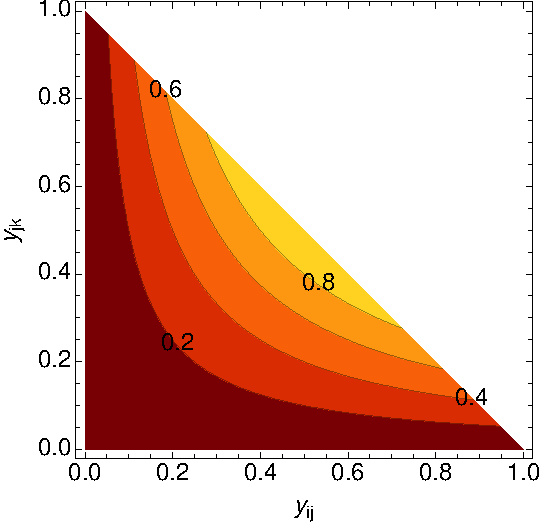
\includegraphics[scale=0.375]{ev1sq} &
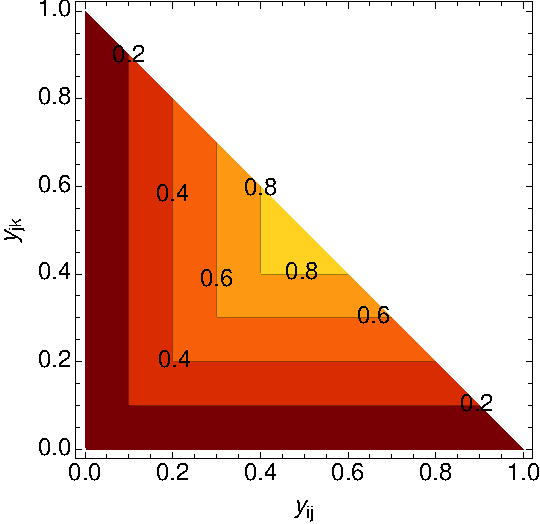
\includegraphics[scale=0.375]{ev2lin} & 
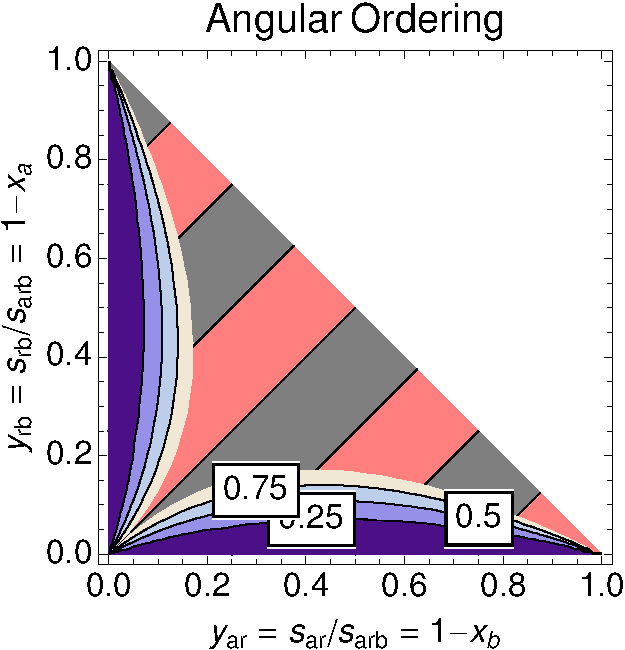
\includegraphics[scale=0.3225]{angord} &
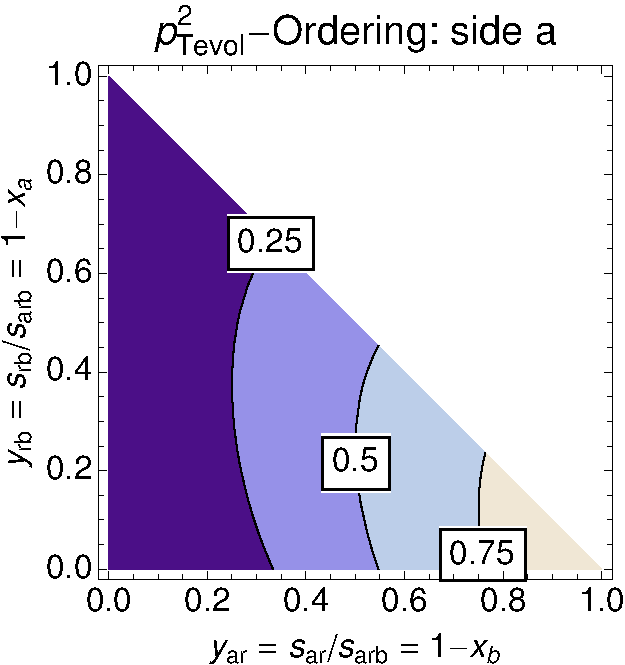
\includegraphics[scale=0.3225]{ptevola} 
\end{tabular}
\caption{A selection of parton-shower evolution variables, represented
as contours over the dipole phase space. Note: the right-most variable
corresponds to evolution of only one of the parents, the one with no
collinear singularity along the bottom of the plot. \label{fig:qe}}
\end{figure}
During the shower
evolution, each model effectively ``sweeps'' over 
phase space in the order implied
by these contours. E.g., a $p_\perp$-ordered dipole shower (leftmost
plot in \figRef{fig:qe}) will treat a hard-collinear branching as
occurring ``earlier'' than a soft one, while a mass-ordered dipole
shower (second plot) will tend to do the opposite. This affects
the tower of virtual corrections generated by each shower model 
via the so-called Sudakov factor, discussed below. Experimental tests
of the subleading aspects of shower models can therefore quite
important, see e.g.~\cite{Fischer:2014bja} for a recent example.

Independently of rewritings and philosophy, 
the real power of \eqRef{eq:eikonal2} lies in the fact
that it is \emph{universal}. Thus, for
\emph{any} process $F$, we can apply \eqRef{eq:eikonal2} in order to
get an approximation for $\dd{\sigma_{F+1}}$. We may then, for instance,  
take our newly obtained expression for $F+1$ as our arbitrary process
and crank \eqRef{eq:eikonal2} again, to obtain an approximation for
$\dd{\sigma_{F+2}}$, and so forth. What we have here is therefore a
very simple recursion relation that can be used to generate approximations to
leading-order cross sections with arbitrary numbers of additional
legs. The quality 
of this approximation is governed by how many terms besides the leading
one shown in \eqRef{eq:eikonal} are included in the game. Including
all possible terms, the most general form for the cross section at 
$F+n\,$ jets, restricted to the phase-space region above some 
infrared cutoff scale $\mu_{\mrm{IR}}$, has the following algebraic structure,
\index{Transcendentality}
\begin{equation}
\sigma_{F+n}^{(0)} = \alpha_s^n \left( 
   \ln^{2n} 
 + \ln^{2n-1} 
 + \ln^{2n-2} 
 + \ldots 
 + \ln{}  
 + {\cal F} \right)  \label{eq:transcend}
\end{equation}
where we use the notation $\ln^\lambda$ without an argument  to denote 
generic functions of \emph{transcendentality} $\lambda$ (the
logarithmic function 
to the power $\lambda$ being a ``typical'' example of a function 
with transcendentality $\lambda$ appearing in cross section expressions, but
also dilogarithms and higher logarithmic functions\footnote{Note: 
due to the theorems 
that allow us, for instance, to rewrite dilogarithms in different
ways with logarithmic and lower ``spillover'' terms, the coefficients at each 
$\lambda$ are only well-defined up to reparametrisation ambiguities
involving the  terms with transcendentality greater than $\lambda$.} of
transcendentality $>1$ should be implicitly understood to belong to
our notation $\ln^\lambda$). The last term, $\cal F$, represents a rational
function of transcendentality 0. We shall also use the nomenclature 
\emph{singular} and \emph{finite} for  the $\ln^\lambda$ and 
${\cal F}$ terms, respectively,  a terminology which reflects their respective
behavior in the limit $\mu_{\mrm{IR}}\to 0$. 

The simplest approximation one can build on \eqRef{eq:transcend}, dropping
all but the leading $\ln^{2n}$ term in the parenthesis, 
is thus the \emph{leading-transcendentality} approximation. This
approximation is better known as 
the DLA (double logarithmic approximation), since it generates the
correct coefficient for terms which have two powers of logarithms for
each power of $\alpha_s$, while terms of lower transcendentalities are not
guaranteed to have the correct coefficients. In so-called LL
(leading-logarithmic) parton shower algorithms, one generally expects
to reproduce the correct coefficients for the $\ln^{2n}$ and
$\ln^{2n-1}$ terms. In addition, several formally subleading
improvements are normally also introduced in such algorithms 
(such as explicit momentum
conservation, gluon polarisation and other 
\index{Spin correlations}%
spin-correlation effects
\cite{Collins:1987cp,Knowles:1988vs,Richardson:2001df},
higher-order coherence effects~\cite{Marchesini:1983bm}, 
renormalisation scale choices
\cite{Catani:1990rr}, finite-width effects \cite{Gigg:2008yc}, etc), 
as a means to improve the agreement
with some of the more subleading coefficients as well, if not in every
phase-space point then at least on average. 
\index{Monte Carlo!Tuning}%
Though LL showers do not magically acquire NLL
(next-to-leading-log) precision from such procedures, one therefore
still expects a significantly better average performance from them 
than from corresponding ``strict'' LL analytical resummations. A side
effect of this is that it is often possible to ``tune'' shower
algorithms to give 
better-than-nominal agreement with experimental distributions, by
adjusting the parameters controlling the treatment of subleading
effects. One should remember, however, that there is a limit to how
much can be accomplished in this way --- at some point, agreement with
one process will only come at the price of disagreement with another,
and at this point further tuning would be meaningless.  

\begin{figure}
\centering
\scalebox{0.9}{
\begin{tabular}{l}
\large\bf F @ LO$\times$LL(non-unitary) \\[2mm]
\begin{loopsnlegs}[c]{p{0.25cm}|ccccc}
 \small 2&~\wbox{\pqcd[2]{0}} & \wbox{\pqcd[2]{1}} & \ldots &
\\[2mm]
 \small 1&~\wbox{\pqcd[1]{0}} & \wbox{\pqcd[1]{1}}  
   & \wbox{\pqcd[1]{2}} & \ldots \\[2mm]
 \small 0&~\gbox{\pqcd[0]{0}} & \ywbox{\pqcd[0]{1}} 
   & \ywbox{\pqcd[0]{2}} &\ywbox{\pqcd[0]{3}} & \ldots \\
\hline
& \small 0 & \small 1 & \small 2 & \small 3 & \ldots
 \end{loopsnlegs}
\end{tabular}}
\caption{Coefficients of the perturbative series covered by LO + LL 
  approximations to higher-multiplicity tree-level matrix elements.
Green (darker) shading represents the full perturbative
  coefficient at the respective $k$ and $\ell$. Yellow (lighter)
  shading represents an LL approximation to it. Half-shaded boxes
  indicate phase spaces in which we are prohibited from integrating
  over the IR singular region, as discussed in
  \secsRef{sec:fixed-order} and \ref{sec:matching}.
\label{fig:LL}}
\end{figure}
Applying such an iterative process on a Born-level cross section, one
obtains the description of the full perturbative series illustrated in
\figRef{fig:LL}. The yellow (lighter) shades
used here for $k\ge 
1$ indicate that the coefficient obtained is not the exact one, but rather an 
approximation to it that only gets its leading singularities
right. However, since this is still only an approximation to
infinite-order \emph{tree-level} cross sections 
(we have not yet included any virtual corrections), 
we cannot yet integrate this approximation over all of
phase space, as illustrated by the yellow boxes being only
half filled in \figRef{fig:LL}; otherwise, the summed total cross section
would still be infinite. This particular approximation would therefore
still appear to be  
very useless indeed --- on one hand, 
it is only guaranteed to get the singular terms right, but on the
other, it does not actually allow us to  integrate over the singular
region. In order to obtain a truly \emph{all-orders} calculation, the
constraint of unitarity must also be explicitly imposed, which
furnishes an approximation to all-orders loop corrections as well.
Let us therefore emphasise that \figRef{fig:LL} is included for
pedagogical purposes only; all resummation calculations, whether
analytical or parton-shower based, include virtual corrections as well
and consequently yield finite total cross sections, as will now be described.

\subsubsection{Step Two: Infinite Loops}

\index{KLN theorem}%
\index{Unitarity}%
Order-by-order unitarity, such as used in the KLN theorem, implies
that the singularities caused by integration over unresolved radiation
in the tree-level matrix elements must be canceled, order by order, by
equal but opposite-sign singularities in the virtual corrections at
the same order. That is, from \eqRef{eq:eikonal2}, we immediately 
know that the 1-loop correction to $\dd{\sigma_F}$ \emph{must} contain a
term, 
\begin{equation}
2\mrm{Re}[{\cal M}_F^{(0)}{\cal M}_F^{(1)*}] \ \supset \ 
- g_s^2 \, N_C \, \left\vert {\cal M}_F^{(0)} \right\vert^2
\, 
\int 
\frac{\dd{s_{ij}}\dd{s_{jk}}}{16\pi^2 s_{ijk}} \left( 
\frac{2s_{ik}}{s_{ij}s_{jk}}~+~\mbox{less singular
  terms}\right)~,\label{eq:eikonalv}
\end{equation}
that cancels the divergence coming from \eqRef{eq:eikonal2}
itself. Further, since this is universally true, we may apply
\eqRef{eq:eikonalv} again to get an approximation to the 
corrections generated by \eqRef{eq:eikonal2} at the next order and so
on. By adding such terms explicitly, order by order, we may now
bootstrap our way around the entire perturbative series, using
\eqRef{eq:eikonal2} to move horizontally and \eqRef{eq:eikonalv} to
move along diagonals of constant $n=k+\ell$. 
\index{Unitarity}
\begin{figure}
\centering
\scalebox{0.9}{
\begin{tabular}{l}
\large\bf F @ LO$\times$LL(unitary)\\[2mm]
\begin{loopsnlegs}[c]{p{0.25cm}|ccccc}
 \small 2&~\ybox{\pqcd[2]{0}} & \ybox{\pqcd[2]{1}} & \ldots & 
\\[2mm]
 \small 1&~\ybox{\pqcd[1]{0}} & \ybox{\pqcd[1]{1}}  
   & \ybox{\pqcd[1]{2}} & \ldots \\[2mm]
 \small 0&~\gbox{\pqcd[0]{0}} & \ybox{\pqcd[0]{1}} 
   & \ybox{\pqcd[0]{2}} &\ybox{\pqcd[0]{3}} & \ldots \\
\hline
& \small 0 & \small 1 & \small 2 & \small 3 & \ldots
 \end{loopsnlegs}
\end{tabular}}
\caption{Coefficients of the perturbative series covered by LO + LL 
  calculations, imposing unitarity order by order for each $n =
  k+\ell$. Green (darker) shading represents the full perturbative
  coefficient at the respective $k$ and $\ell$. Yellow (lighter)
  shading represents an LL approximation to it. 
\label{fig:LLu}}
\end{figure}
Since real-virtual cancellations are now explicitly restored, we may
finally extend the integrations over all of phase space, resulting in
the picture shown in \figRef{fig:LLu}. 

The picture shown in \figRef{fig:LLu}, not the one in \figRef{fig:LL}, 
corresponds to what is actually done in
\emph{resummation} calculations, both of the analytic and
parton-shower types\footnote{In the way these calculations are 
formulated in practice, they
in fact rely on one additional property, called exponentiation, that allows us
to move along straight vertical lines in the loops-and-legs diagrams. However, 
since the two different directions furnished by \eqsRef{eq:eikonal2} and
\eqref{eq:eikonalv} are already sufficient to move freely in the
full 2D coefficient space, we shall use exponentiation
without extensively justifying it here.}.
\index{Unitarity}
Physically, there is a significant and intuitive meaning to the imposition of
unitarity, as follows. 

\index{Jets}
\index{Inclusive cross sections}
\index{Exclusive cross sections}
\index{Event evolution|see{Evolution}}
\index{Evolution}
Take a jet algorithm, with some measure of jet resolution, $Q$, and
apply it to an arbitrary sample of events, say dijets. At a very crude
resolution scale, corresponding to a high value for $Q$, 
you find that everything is clustered back to a dijet configuration,
and the 2-jet cross section is equal to the total inclusive cross
section,
\begin{equation}
\sigma_\mrm{tot} = \sigma_{F;\mrm{incl}} ~.
\end{equation}
At finer resolutions, decreasing $Q$, you see that 
some events that were previously classified as 2-jet events contain
additional, lower-scale jets, that you can now resolve, and hence
those events now migrate to the 3-jet bin, while the total inclusive
cross section of course remains unchanged,
\index{Inclusive cross sections}
\index{Exclusive cross sections}
\index{Evolution}
\begin{equation}
\sigma_\mrm{tot} = \sigma_{F;\mrm{incl}} = \sigma_{F;\mrm{excl}}(Q)
+ \sigma_{F+1;\mrm{incl}}(Q)~, \label{eq:incexc}
\end{equation}
where ``incl'' and ``excl'' stands for inclusive and exclusive cross
sections\footnote{$F$ \emph{inclusive} $=$ $F$ plus
  anything. $F$ \emph{exclusive} $=$ $F$ and only
  $F$. Thus, $\sigma_{F;\mathrm{incl}}=\sum_{\mrm{k}=
    0}^{\infty}\sigma_{F+k;\mrm{excl}}$},  
respectively, 
and the $Q$-dependence in the two terms on the 
right-hand side must cancel so that the total inclusive cross
section is independent of $Q$. Later, some 3-jet events now migrate 
further, to 4 and higher jets, 
while still more 2-jet events migrate \emph{into} the 3-jet
bin, etc. For arbitrary $n$ and $Q$, we have
\index{Inclusive cross sections}
\index{Exclusive cross sections}
\index{Evolution}
\begin{equation}
\sigma_{F+n;\mrm{incl}}(Q) = \sigma_{F;\mrm{incl}}
- \sum_{m=0}^{n-1} \sigma_{F+m;\mrm{excl}}(Q)~. 
\end{equation}
This equation expresses the trivial fact that the cross section for
$n$ or more jets can be computed as the total inclusive cross section for $F$
minus a sum over the cross sections for $F$ + exactly $m$ jets including
all $m<n$. On the theoretical side, it is these negative terms which must
be included in the calculation, for each order $n=k+\ell$, to restore
unitarity. Physically, they 
express that, at a given scale $Q$, each event will be classified
as having \emph{either} 0, 1, 2, or whatever jets. Or, equivalently,
for each event we gain in the 3-jet bin as $Q$ is lowered, we must loose one
event in the 2-jet one; the negative contribution to the 2-jet bin
is exactly minus the integral of the positive contribution to the
3-jet one, and so on. 
\index{Detailed balance}
\index{Evolution}
We may perceive of this \emph{detailed balance}
 as an \emph{evolution} of the event structure with $Q$, for each 
event, which is effectively what is done in parton-shower
algorithms, to which we shall return in \SecRef{sec:Markov}.

\subsection{Perturbation Theory with Markov Chains \label{sec:Markov}}
Consider again the Born-level cross section for an arbitrary hard process,
$F$, differentially in an arbitrary infrared-safe observable $\cal O$,
as obtained from \eqRef{eq:fixed-order}:
\begin{equation}
\left.   \frac{\dd{\sigma^{(0)}_F}}{\dd{\cal O}}\right\vert_{\mbox{\textcolor{black}{Born}}}
 = \int \dPS{F} \ |{\cal M}_F^{(0)}|^2 \ \delta({\cal
   O}-{\cal O}(\PS{F}))~,
\label{eq:starting}
\end{equation}
where the integration runs over the full final-state on-shell phase space of
$F$ (this expression and those below would also apply to hadron collisions
were we to include integrations over the parton distribution functions
in the initial state), and the $\delta$ function projects out a
1-dimensional slice defined by $\cal O$ evaluated on the 
set of final-state momenta which we denote $\PS{F}$.
 
\index{Evolution}
\index{Parton showers}
To make the connection to parton showers, 
we insert an operator, ${\cal S}$, that acts on the Born-level
final state \emph{before} the observable is evaluated, i.e., 
\begin{equation}
\left.   \frac{\dd{\sigma_F}}{\dd{\cal
    O}}\right\vert_{\mbox{\textcolor{black}{${\cal S}$}}}
 = \int \dd{\Phi_F} \ |{\cal M}_F^{(0)}|^2 \ {\cal S}(\PS{F},{\cal O})~.
\end{equation}
Formally, this operator --- the evolution operator --- will be
responsible for generating all (real and virtual) 
higher-order corrections to the Born-level expression.
The measurement $\delta$ function appearing explicitly in
\eqRef{eq:starting} is now implicit in ${\cal S}$.

\index{Evolution}
\index{Factorisation!Factorisation scale}
\index{Parton showers}
\index{Parton showers!Evolution variable}
Algorithmically, parton showers cast $\cal S$ as an iterative Markov
(i.e., history-independent) chain, 
with an evolution parameter, $Q_E$, that formally 
represents the factorisation scale of the event, below which all
structure is summed over inclusively. Depending on the particular
choice of shower algorithm, $Q_E$ may be defined as a parton
virtuality (virtuality-order showers), as a transverse-momentum scale
\index{pT-ordering@$p_\perp$-ordering}
\index{Transverse-momentum-ordering|see{$p_\perp$-ordering}}
($p_\perp$-ordered showers), or as a combination of
\index{Angular ordering}
energies times angles (angular ordering). Regardless of the specific
form of $Q_E$, 
the evolution parameter will go towards zero as the Markov chain
develops, and the event structure
will become more and more exclusively resolved. 
\index{Parton showers!Infrared cutoff|see{Hadronisation scale}}
\index{Hadronisation scale}
A transition from a
perturbative evolution to a non-perturbative one can also be
inserted, when the evolution reaches an appropriate scale, typically 
around 1~GeV. This scale, called the \emph{hadronisation scale}, thus 
represents the lowest perturbative scale that can appear in the
calculations, with all perturbative corrections below it
summed over inclusively.

Working out the precise form that $\cal S$ must have in order to give the
correct expansions discussed in \secRef{sec:parton-showers} takes a
bit of algebra, and is beyond the scope we aim to cover in these
lectures. Heuristically, the procedure is as follows. 
We noted that the singularity structure of QCD is universal
and that at least its first few terms are known to us. We also saw
that we could iterate 
that singularity structure, using universality and unitarity, 
thereby bootstrapping our way around the entire perturbative
series. This was illustrated by 
\figRef{fig:LLu} in \secRef{sec:parton-showers}. 

\index{Evolution}
\index{Markov chains}
Skipping intermediate steps, the form of the all-orders pure-shower
Markov chain, for the evolution of an event between two scales $Q_{1}
> Q_E > Q_{2}$, is,  
\begin{equation}\begin{array}{rcl}
\displaystyle \hspace*{-1mm} {\cal S}(\PS{F},Q_{1},Q_{2},\obs) \hspace*{-1mm}
&  \hspace*{-1mm}= \hspace*{-1mm} &\displaystyle \hspace*{-1mm}
  \underbrace{
\Delta(\PS{F},Q_{1},Q_{2})\ 
\delta\left(\obs-\obs(\PS{F})\right) 
}_{\mbox{$F+0$ exclusive above $Q_{2}$}}\\[9mm]
& & \hspace*{-1.2cm}+ \displaystyle 
\underbrace{
\sum_r \int_{Q_{E2}}^{Q_{E1}}
\frac{\dPS[r]{F+1}}{\dPS{F}} 
\ S_r(\PS{F+1}) \ \Delta(\PS{F},Q_{1},Q_{F+1})
 \ {\cal S}(\PS{F+1},Q_{F+1},Q_{2},\obs)}_{\mbox{$F+1$ inclusive above $Q_{2}$}}
~,\label{eq:markov} \hspace*{-1mm}
\end{array}
\end{equation}
\index{Sudakov factor}
\index{Parton showers!Sudakov factor}
with the so-called \emph{Sudakov factor},
\begin{equation} 
\Delta(\PS{F},Q_{1},Q_{2}) = \exp\left[-\sum_r\int_{Q_{2}}^{Q_{1}} 
\frac{\dPS[r]{F+1}}{\dPS{F}} S_r(\PS{F+1}) \right]~, \label{eq:sudakov}
\end{equation}
defining the probability that there is \emph{no evolution} (i.e., no
emissions) between the scales $Q_{1}$ and $Q_{2}$, according to the
\emph{radiation functions} $S_r$ to which we shall return below. 
\index{Markov chains}
The term on the first line of
\eqRef{eq:markov} thus represents all events that \emph{did not}
evolve as the resolution scale was lowered from $Q_{1}$ to $Q_{2}$,
while the second line contains a sum and phase-space integral over
those events that \emph{did} evolve --- including the insertion of ${\cal
  S}(\PS{F+1})$ representing the possible further evolution of the
event and completing the iterative definition of the Markov chain. 

The factor $\dPS[r]{F+1}/\dPS{F}$
defines the chosen phase space factorisation. Our favorite is the
so-called dipole-antenna factorisation, whose principal virtue is that
it is the simplest Lorentz invariant 
factorisation which is simultaneously exact over
all of phase space while only involving on-shell momenta. For
completeness, its form is
\begin{equation}  
\frac{\dPS[r]{F+1}}{\dPS{F}} = \frac{\dPS[r]{3}}{\dPS{2}} =
\dd{s_{a1}} \dd{s_{1b}} \frac{\dd{\phi}}{2\pi} \frac{1}{16\pi^2
  s_r}~, \label{eq:phasespace} 
\end{equation}
which involves just one color-anticolor pair for each $r$, with
invariant mass squared $s_r = (p_a+p_1+p_b)^2$. 
Other choices, such as purely collinear ones (only exact in the
collinear limit \emph{or} involving explicitly off-shell momenta), 
more global ones involving all partons in the event (more complicated,
in our opinion), or less global ones with a single parton playing the
dominant role as emitter, are also possible, again depending 
on the specific algorithm considered.

The radiation functions $S_r$ obviously play a crucial role in these
equations, driving the emission probabilities. For example, if 
$S_r \to 0$, then  $\Delta \to \exp(0) = 1$ and all events stay in the
top line of \eqRef{eq:markov}. Thus, in regions of phase  
space where $S_r$ is small, there is little or no evolution. 
Conversely, for $S_r\to \infty$, we have $\Delta\to 0$, implying that \emph{all}
events evolve. 
One possible choice for the radiation functions $S_r$ was
implicit in \eqRef{eq:eikonal2}, in which we took them to include only
the leading 
(double) singularities, with $r$ representing color-anticolor
pairs. In general, the shower
may exponentiate the entire set of universal singular terms, or only
a subset of them (for example, the terms leading in the number of colors
$N_C$), which is why we here let the explicit form of $S_r$ be
unspecified. 
\index{DGLAP kernels}%
Suffice it to say that 
in traditional parton showers, $S_r$ would simply be the DGLAP
splitting kernels (see, e.g., \cite{Dissertori:2003pj}), 
\index{Antennae}%
while they would be so-called dipole or antenna radiation
functions in the various dipole-based approaches to QCD 
(see, e.g.,
\cite{Azimov:1986sf,Gustafson:1987rq,Catani:1996vz,GehrmannDeRidder:2005cm,Giele:2007di,Schumann:2007mg,Giele:2011cb,LopezVillarejo:2011ap}).   

The procedure for how to technically ``construct'' a shower algorithm
of this kind, using random numbers to generate scales distributed according to
\eqRef{eq:markov}, is described more fully in \cite{Giele:2011cb},
using a notation that closely parallels the one used here. The
procedure is also described at a more technical level in the review
\cite{Buckley:2011ms}, though using a slightly different
notation. Various aspects of the Sudakov veto algorithm are discussed
in \cite{Platzer:2011dq,Lonnblad:2012hz,Mrenna:2016sih}.
\index{Monte Carlo!Pedagogical introduction}%
Finally, pedagogical introduction to Monte Carlo
methods in general can be found in \cite{James:1980yn,Weinzierl:2000wd}. 

\subsection{Decays of Unstable Particles \label{sec:decays}}
\index{Resonance decays}%
\index{Monte Carlo!Decay distributions}%
In most BSM processes and some SM ones, an important aspect of the
event simulation is how decays of short-lived particles, such as top
quarks, EW and Higgs bosons, and new BSM resonances, are
handled. We here briefly summarise the spectrum of possibilities, but
emphasise that there is no universal standard. Users are advised to check
 whether the treatment of a given code is adequate for the physics
study at hand. 

The appearance of an unstable resonance as a physical particle
at some intermediate stage of the event generation implies that its
production and decay processes are treated as being factorised. 
\index{Narrow width approximation}%
This is called the \emph{narrow width approximation} and is 
valid up to corrections of order $\Gamma/m_0$, with $\Gamma$
the width and $m_0$ the pole mass of the particle. 
States whose widths are a substantial fraction
of their mass should not be treated in this way, but 
rather as intrinsically virtual internal propagator lines. 

For states treated as physical particles, two aspects are relevant:
the mass distribution of the decaying particle itself and the
distributions of its decay products. For the mass distribution, 
the simplest is to use a 
$\delta$ function at $m_0$. The next level up, typically
used in general-purpose Monte Carlos, 
\index{Breit-Wigner distribution}%
is to use a Breit-Wigner distribution (relativistic or
non-relativistic), which formally resums  higher-order virtual corrections to
the mass distribution. Note, however, that this 
still only generates an improved picture for \emph{moderate} fluctuations
away from $m_0$. Similarly to above, particles 
that are significantly off-shell (in units of $\Gamma$) should not be
treated as resonant, but rather as internal off-shell propagator
lines. In most Monte Carlo codes, some further refinements are also 
included, for instance
by letting $\Gamma$ be a function of $m$ (``running widths'') and by
limiting the magnitude of the allowed fluctuations away from
$m_0$. See also \cite{Seymour:1995qg} for an elaborate discussion of the
Higgs boson lineshape. 

For the distributions of the decay products, the simplest treatment is
again to assign them their respective $m_0$ values, with a uniform
(i.e., isotropic, or ``flat'')
phase-space distribution. A more sophisticated treatment distributes
the decay products according to the differential decay matrix
elements, capturing at least the internal dynamics and helicity
structure of the decay process, including EPR-like correlations. 
\index{Spin correlations}%
Further refinements include polarisations of the external 
states~\cite{Collins:1987cp,Knowles:1988vs,Richardson:2001df} (see
also \cite{Stelzer:1995gc,Parke:1996pr,Smillie:2005ar} 
for phenomenological studies)
 and assigning the decay products their own
Breit-Wigner distributions, the latter of which 
opens the possibility to  include also intrinsically off-shell decay
channels, like $H\to W W^*$. Please refer to the physics manual of the
code you are using and/or make simple cross checks like plotting the
distribution of phase-space invariants it produces.

\index{Resonance decays}%
During  subsequent showering of the decay products, 
most parton-shower models will preserve the total invariant 
mass of each resonance-decay system separately, 
so as not to skew the original resonance shape.

%%% Should write a section here with more elaborate comments on the
%%% treatment of Breit-Wigner shapes and running widths, radiation
%%% from unstable particles. Top mass?

